\documentclass[a4paper,14pt,oneside,openany]{memoir}

%%% Задаем поля, отступы и межстрочный интервал %%%

\usepackage[left=10mm, right=15mm, top=20mm, bottom=20mm]{geometry} 

\usepackage[english, russian]{babel}    
\usepackage{longtable,ltcaption}                    % Длинные таблицы
\usepackage{multirow,makecell}                      % Улучшенное форматирование таблиц
\usepackage{booktabs}                               % Еще один пакет для красивых таблиц
\usepackage{soulutf8}                               % Поддержка переносоустойчивых подчёркиваний и зачёркиваний
\usepackage{icomma}                                 % Запятая в десятичных дробях
\usepackage{hyphenat}                               % Для красивых переносов
\usepackage{textcomp}                               % Поддержка "сложных" печатных символов типа значков иены, копирайта и т.д.
\usepackage[version=4]{mhchem}                      % Красивые химические уравнения
\usepackage{amsmath} 

\usepackage[utf8]{inputenc}

\usepackage{amsthm}
\usepackage{amssymb}
\usepackage{enumerate}
\usepackage{stmaryrd}
\usepackage{cmll}
\usepackage{mathrsfs}
\usepackage{proof}
\usepackage{tikz}
\usepackage{multicol}
\usepackage{mathabx}
\usepackage{pdflscape}
\usepackage{listings}
\usepackage{xcolor}

%opening
\title{}
\author{}

\definecolor{codegreen}{rgb}{0,0.6,0}
\definecolor{codegray}{rgb}{0.5,0.5,0.5}
\definecolor{codepurple}{rgb}{0.58,0,0.82}

\lstdefinestyle{mystyle}{
	keywordstyle=\color{codepurple},
	numberstyle=\tiny\color{codegray},
	stringstyle=\color{codegreen},
	basicstyle=\ttfamily\footnotesize,
	breakatwhitespace=false,         
	breaklines=true,                 
	captionpos=b,                    
	keepspaces=true,                 
	numbers=left,                    
	numbersep=5pt,                  
	showspaces=false,                
	showstringspaces=false,
	showtabs=false,                  
	tabsize=2
}

\lstset{style=mystyle}


\begin{document}

\thispagestyle{empty}

\begin{center}
	
	Национальный исследовательский университет ИТМО\\
	Факультет информационных технологий и программирования\\
	Прикладная матеметика и информатика\\
	
	\vspace{20pt}
	
\end{center}

\vfill

\begin{center}
	\textbf {\fontsize{100}{120}\selectfont Методы оптимизации
	} \\  
	Отчет по лабораторной работе №3
	
\end{center}

\vfill

\begin{flushright}
	
	\hfill {
		Работу \\
		выполняли: \\
		Кольченко Антон М32371 \\ 
		Гайнанов Ильдар М32371 \\ 
		Муфтиев Руслан М32331\\ 
	}
	\vspace{20pt}
	
\end{flushright}

\vfill

\begin{center}
	Санкт-Петербург\\
	2023
\end{center}

\chapter*{Введение}
\textbf{Постановка задачи:}

\begin{enumerate}
\item Реализовать методы Gauss-Newton и Powell Dog Leg для решения нелинейной регрессии. Сравнить эффективность с методами, реализованными в предыдущих работах.
\item Реализовать метод BFGS и исследовать его сходимость при минимизации различных функций. Сравнить с другими реализованными методами.
\item Реализовать и исследовать метод L-BFGS.
\end{enumerate}

\chapter{Теоретическая часть}
\section{Методы регрессии}
Вход: множество точек $\{(x_i, y_i)\ |\ x_i, y_i \in \mathbb{R}\}$\\
Выход: зависимость $y$ от $x$, выраженная как $\sum_{i=0}^{p} c_ix^i + \epsilon.$ \\
Далее:
$w := \{c_1, c_2, ... c_p\}$ \\
$r(w) := y - f(x, w)$, где $f$ - функция, для которой мы восстанавливаем коэффиценты.

\subsection{Метод Гаусса-Ньютона}

Принцип работы: 

Метод Гаусса-Ньютона находит решение задачи поиска наименьших квадратов, используя якобиану $J$ функции ошибки. Он основан на методе Ньютона, который использует гессиан (матрицу вторых производных), который слишком долго высчитывается для того, чтобы быть применимым в реальной жизни. Вместо этого гессиан апроксимируется сочетанием якобианов (матриц первой производной).

Алгоритм:
\begin{enumerate}
	\item $J := J_r(w)$.
	\item $\delta = -(J^TJ)^{-1}J^Tr(w)$.
	\item $w = w + \delta$.
	\item Повторять шаги, пока $|\Delta MSE| > \varepsilon$.
\end{enumerate}

\subsection{Метод Powell's Dog Leg}

Принцип работы: 

Метод Dog Leg объединяет градиентный спуск и метод Гаусса-Ньютона для рещения задачи наименьших квадратов. Более того, в алгоритме используется доверительная область $TR$ с радиусом $R$, которой будут ограничены размеры шага алгоритма. 

$TR_w := \{w': dist(w, w') < R\}$

Алгоритм:
\begin{enumerate}
	\item $J := J_r(w)$
	\item $\delta_{Gauss-Newton} = -(J^TJ)^{-1}J^Tr(w)$.
	\item $\delta_{Gradient Descent} = -J^Tr(w)$.
	\item $t = -\dfrac{\delta_{Gradient Descent}^T\cdot J^T \cdot r(w)}{||J\cdot\delta_{Gradient Descent}||^2}$.
	\item $\delta = \begin{cases}
		\delta_{Gauss-Newton}\quad\quad \delta_{Gauss-Newton} \in TR_w, \\
		R\cdot\dfrac{\delta_{Gradient Descent}}{||\delta_{Gradient Descent}||} \quad\quad \delta_{Gauss-Newton} \not\in TR_w,\ \delta_{Gradient Descent}\not\in TR_w, \\
		t\delta_{Gradient Descent} + R(\delta_{Gauss-Newton} - t\cdot \delta_{Gradient Descent}) \quad\quad \text{иначе}.
	\end{cases}$
	\item Повторять шаги, пока $|\Delta MSE| > \varepsilon$.
\end{enumerate}

\section{BFGS, L-BFGS}

Вход: функция $f:\mathbb{R}^n \rightarrow \mathbb{R}$, стартовая точка $x = (x_1,x_2,...,x_n)$, точность $\varepsilon$. \\
Выход: найденная точка локального минимума
\subsection {BFGS}

Принцип работы: 

В BFGS и производных мы пользуемся не только градиентом (т.е. вектором первых производных), но и гессианом (матрицей вторых производных). Однако гессиан вычисляется слишком долго, поэтому будем его апроксимировать (а точнее не его, а обратную к нему матрицу). 

$C$ - апроксимация $H^{-1}$. $C^{[0]}$ можно задать как честный $H^{-1}$ или как $I$.
$A \times B$ - здесь внешнее произведение $A$ и $B$.
Алгоритм:
\begin{enumerate}
	\item $p^{[k + 1]} = -C^{[k]} \cdot \nabla f(x^{[k]})$.
	\item $\delta^{[k + 1]} = \alpha p^{[k + 1]}$, где $\alpha$ находится по признаку Вольфе.
	\item $x^{[k + 1]} = x^{[k]} + \delta$ 
	\item $y^{[k + 1]} =  \nabla f(x^{[k + 1]}) - \nabla f(x^{[k]})$
	\item $\rho^{[k + 1]} = \dfrac{1}{(y^{[k + 1]})^T \cdot\delta^{[k + 1]}}$
	\item $C^{[k + 1]} = (I - \rho \cdot \delta^{[k + 1]} \times (y^{[k + 1]})^T)C^{[k]}(I - \rho \cdot y^{[k + 1]} \times (\delta^{[k + 1]})^T) + \rho \cdot \delta^{[k + 1]} \times (\delta^{[k + 1]})^T$
	\item Повторять шаги, пока  $||\nabla f(x^{[k]})|| > \varepsilon$.
\end{enumerate}

\subsection {L-BFGS}

Вход: дополнительно $m$ - количество предыдущих сохраненных итераций алгоритма.
Принцип работы: 


У BFGS есть существенный недостаток - расход памяти, т.к. гессиан занимает $O(n^2)$ памяти. L-BFGS частично жертвует точностью, чтобы занимать $O(mn)$ памяти $(m << n)$.

$C$ - апроксимация $H^{-1}$. $C^{[0]}$ можно задать как честный $H^{-1}$ или как $I$.
$A \times B$ - здесь внешнее произведение $A$ и $B$.
Алгоритм:
\begin{enumerate}
	\item $q = \nabla f(x^{[k]})$.
	\item Для каждого $i = k - 1, k - 2, ..., k - m$: \\
	$\quad\quad\alpha^{[i]} = \rho^{[i]} \cdot (s^{[i]})^T \times q$ \\
	$\quad\quad q = q - \alpha^{[i]} \cdot y^{[i]}$.
	\item $\gamma = \dfrac{(s^{[k]})^T\cdot y^{[k]}}{(y^{[k]}) \cdot y^{[k]}}$	.
	\item $C = \gamma I$.
	\item $z = Cq$.
	\item Для каждого $i = k - m, k - m + 1, ..., k - 1$: \\
		$\quad\quad\beta^{[i]} = \rho^{[i]} \cdot (y^{[i]})^T \times z$ \\
		$\quad\quad z = z + s^{[i]} \cdot (\alpha^{[i]} - \beta^{[i]})$. 
	\item $p^{[k + 1]} = -z$
	\item $\delta^{[k + 1]} = \alpha p^{[k + 1]}$, где $\alpha$ находится по признаку Вольфе.
	\item $x^{[k + 1]} = x^{[k]} + \delta$ 
	\item $y^{[k + 1]} =  \nabla f(x^{[k + 1]}) - \nabla f(x^{[k]})$
	\item $\rho^{[k + 1]} = \dfrac{1}{(y^{[k + 1]})^T \cdot\delta^{[k + 1]}}$
	\item Повторять шаги, пока  $||\nabla f(x^{[k]})|| > \varepsilon$.
\end{enumerate}


\chapter{Практическая часть}
 
\section{Методы решения задачи нелинейной регрессии}
\subsection{Реализация метода Гаусса-Ньютона}
\begin{lstlisting}[language=Python, caption=Метод Гаусса-Ньютона]
	def gauss_newton(p, points, num_iters=100):
	    w = np.zeros(p+1)
	    A = np.array([[x ** i for i in range(p + 1)] for x in points[:, 0]])
	    x = points[:, 0]
	    y = points[:, 1]
	    r = lambda w: y - np.array(sum(w[i] * x ** i for i in range(p + 1)))
	    err = lambda w: sum(map(lambda ri: ri ** 2, r(w)))
	    for cnt in range(num_iters):
	        J = jacobian(r, w)
	
	        delta = -(np.linalg.inv(J.T @ J) @ J.T @ r(w))
	        
	        prev_err = err(w)
	        w += delta 
	        # print(sum(w[i] * x ** i for i in range(p + 1)))
	
	        if abs(err(w) - prev_err) < 1e-5:
	            break
	
	    return w, cnt
	
\end{lstlisting}

\newpage

\subsection{Реализация метода Dog Leg}
\begin{lstlisting}[language=Python, caption=Метод Powell's Dog Leg]
	def dog_leg(p, points, trust_region=1, num_iters=100):
		def step(J, r: np.ndarray):
		        gn_delta = -np.linalg.inv(J.T @ J) @ J.T @ r # gauss-newton
		        if np.linalg.norm(gn_delta) <= trust_region:
		            return gn_delta
		        
		        st_delta = -J.T @ r # gradient descent
		        if np.linalg.norm(st_delta) > trust_region:
		            return st_delta / np.linalg.norm(st_delta) * trust_region
		
		        t = (np.linalg.norm(st_delta) / np.linalg.norm(J @ st_delta)) ** 2
		        return t * st_delta + trust_region * (gn_delta - t * st_delta)
		
		    w = np.zeros(p+1)
		    A = np.array([[x ** i for i in range(p + 1)] for x in points[:, 0]])
		    x = points[:, 0]
		    y = points[:, 1]
		    r = lambda w: y - np.array(sum(w[i] * x ** i for i in range(p + 1)))
		    err = lambda w: sum(map(lambda ri: ri ** 2, r(w)))
		    for cnt in range(num_iters):
		        J = jacobian(r, w)
		
		        delta = step(J, r(w))
		
		        prev_err = err(w)
		        w += delta 
		
		        if abs(err(w) - prev_err) < 1e-5:
		            break
		
		
		    return w, cnt
	
\end{lstlisting}

\begin{figure}[ht]
	\centering
	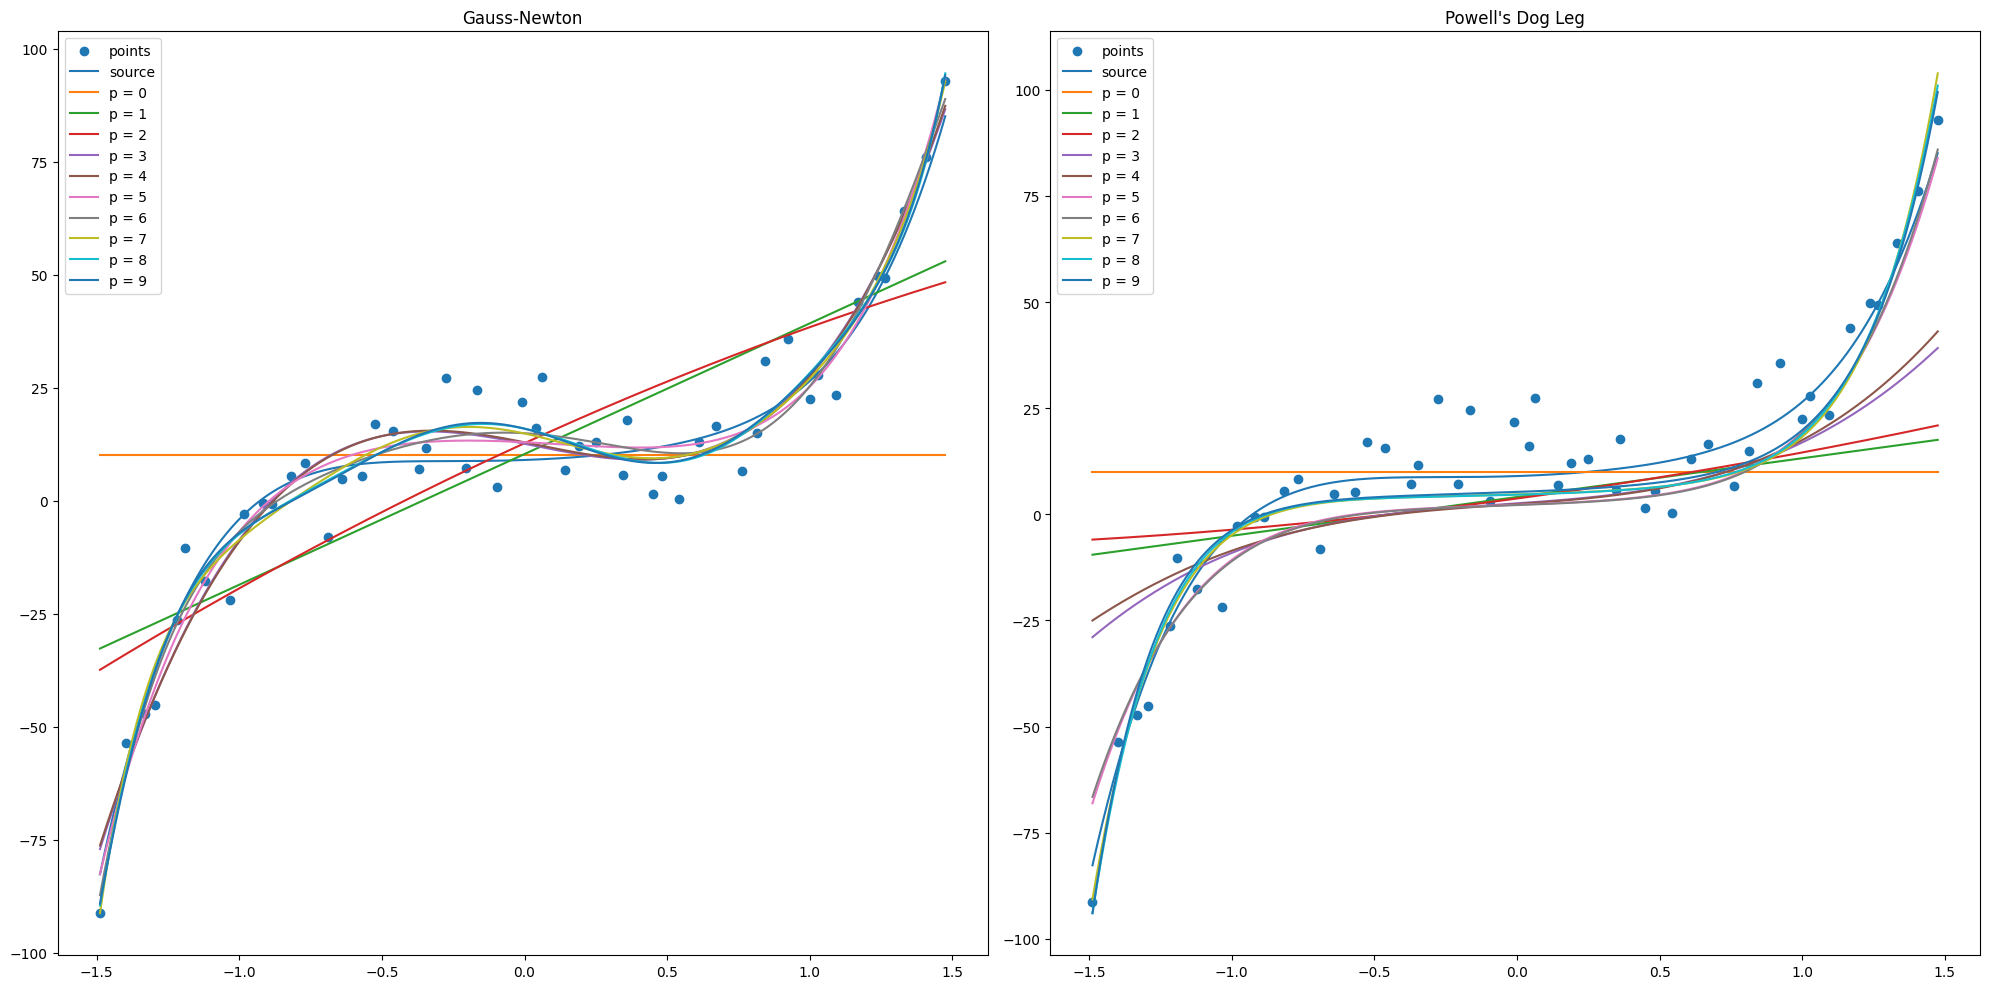
\includegraphics[width=1\textwidth]{img/3_1_1.png}
    \caption{График сходимости методов на полиномиальной функции}
\end{figure}

\newpage

\subsection{Сравнение}

\begin{figure}[ht]
	\centering
	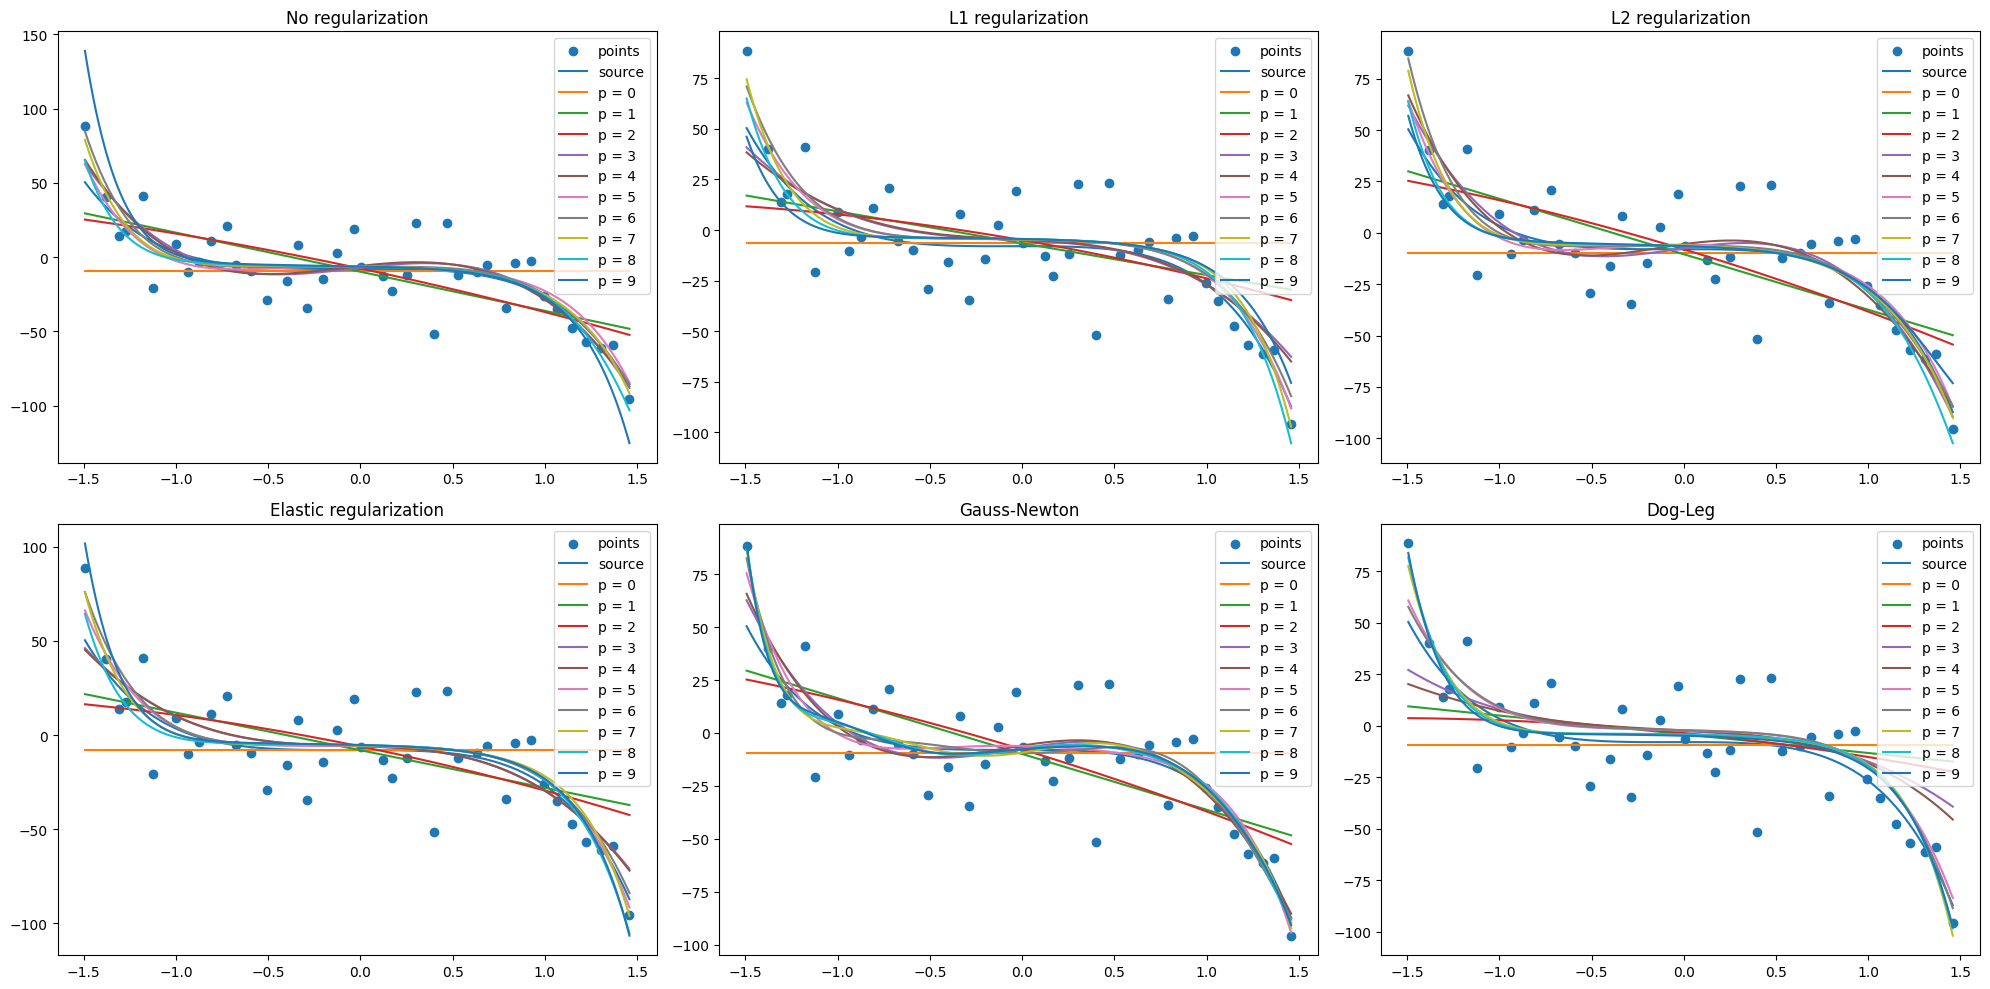
\includegraphics[width=1\textwidth]{img/3_2_2.png}
    \caption{График сходимости методов на полиномиальной функции}
\end{figure}

\begin{figure}[ht]
	\centering
	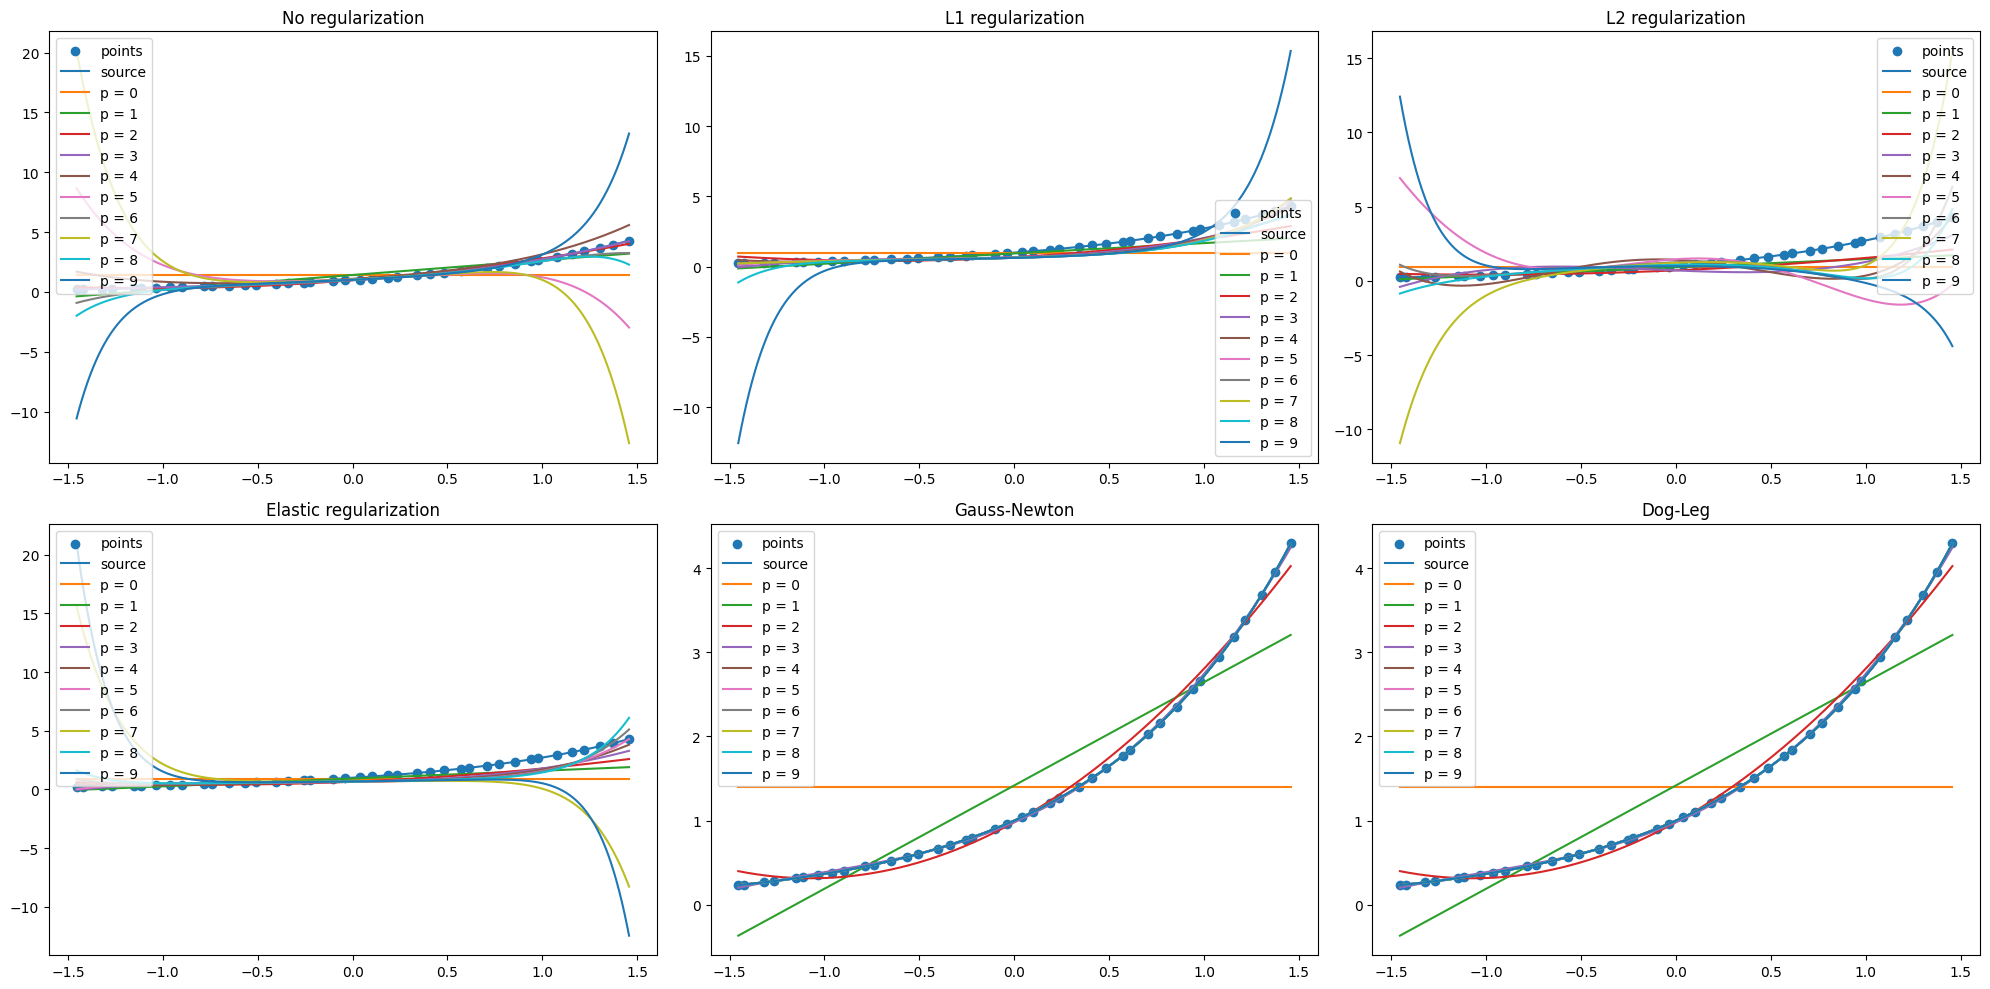
\includegraphics[width=1\textwidth]{img/3_2_3.png}
    \caption{График сходимости методов на экспоненциальной функции}
\end{figure}

\subsection{Выводы}

\begin{itemize}
\item Метод Гаусса-Ньютона сходится быстрее всех остальных, даже чем Dog Leg. Полиномиальные регрессии он нередко находит за 1 итерацию.
\item Тем не менее, метод Гаусса-Ньютона имеет склонность к переобучению, в отличие от Dog Leg.
\item Оба метода умеют решать задачу поиска регрессии для функций, которые даже не являются полиномиальными.
\end{itemize}

\newpage

\section{BFGS, L-BFGS}
\subsection{Реализация}



\begin{lstlisting}[language=Python, caption=Реализация BFGS]
	def fast_bfgs_gd(f, x, lim=500):
	    n = len(x)
	    points = []
	    g = None
	    C = np.linalg.inv(hessian(f, x))
	    points.append(x)
	    while True:
	        if g is None:
	            g = grad(f, x)
	
	        if np.linalg.norm(g) < eps:
	            break
	
	        p = -C @ g
	
	        alpha = find_wolfe(f, x, p)
	        delta = p * alpha
	        x = x + delta
	        points.append(x)
	
	        if (len(points) > lim):
	            break
	
	        newg = grad(f, x)
	        y = newg - g
	        g = newg
	
	        I = np.eye(n)
	        rho = 1 / (y.T @ delta)
	        C = (I - rho * np.outer(delta, y.T)) @ C @ (I - rho * np.outer(y, delta.T)) + \
	            rho * np.outer(delta, delta.T)
	
	    return np.array(points)
\end{lstlisting}

\begin{lstlisting}[language=Python, caption=Реализация L-BFGS]
	def l_bfgs_gd(f, x, m=8, lim=500):
	    n = len(x)
	    points = []
	    rho_q = deque(maxlen=m)
	    s_q = deque(maxlen=m)
	    y_q = deque(maxlen=m)
	    g = None
	    points.append(x)
	    while True:
	        if g is None:
	            g = grad(f, x)
	
	        if np.linalg.norm(g) < eps:
	            break
	
	        alpha_q = []
	
	        q = g
	        for s, rho, y in zip(reversed(s_q), reversed(rho_q), reversed(y_q)):
	            alpha = rho * np.outer(s.T, q)
	            alpha_q.append(alpha)
	            q = q - alpha @ y
	
	        try:
	            gamma = (s_q[-1].T @ y_q[-1]) / (y_q[-1].T @ y_q[-1])
	            H = gamma * np.eye(n)
	        except IndexError:
	            H = np.linalg.inv(hessian(f, x))
	
	        z = H @ q
	
	        for s, rho, y, alpha in zip(s_q, rho_q, y_q, reversed(alpha_q)):
	            beta = rho * np.outer(y.T, z)
	            z = z + s @ (alpha - beta)
	
	        p = -z
	        alpha = find_wolfe(f, x, p)
	        delta = p * alpha
	        s_q.append(delta)
	        x = x + delta
	        points.append(x)
	
	        if (len(points) > lim):
	            break
	
	        newg = grad(f, x)
	        y = newg - g
	        y_q.append(y)
	        g = newg
	
	        rho = 1 / (y.T @ delta)
	        rho_q.append(rho)
	
	    return np.array(points)
	
\end{lstlisting}
    
   
    
	\subsection {Сравнение}

	\begin{figure}[ht]
		\centering
		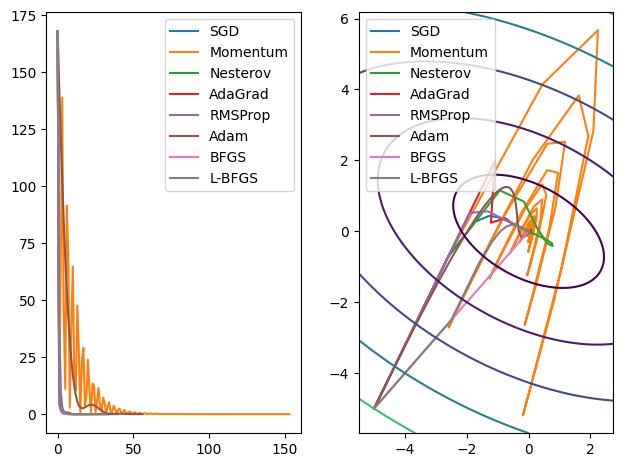
\includegraphics[width=0.65\textwidth]{img/3_3_1.png}
  \caption{Демонстрация графиков сходимости различных модификаций стохастического градиентного спуска}
  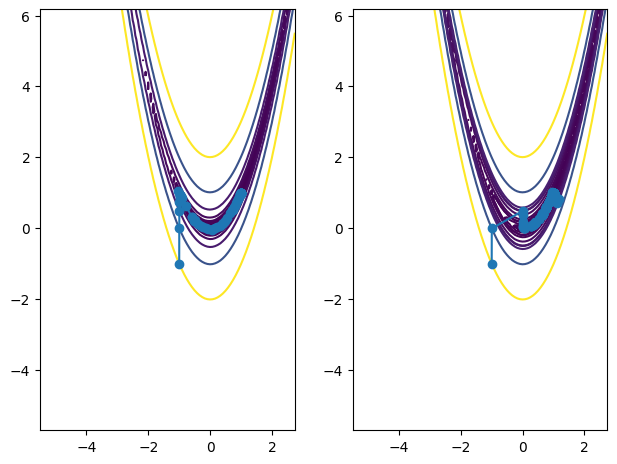
\includegraphics[width=0.65\textwidth]{img/3_3_2.png}
    \caption{Демонстрация графиков сходимости BFGS и L-BFGS на функции Розенброка}
	\end{figure}
	
	
	\begin{table}
	Рассмотрим вычислительные затраты методов $(dim = 100)$:
	\centering
	\begin{tabular}{|c|c|c|c|c|c|c| }
	\hline
	& time, s & iters & mem usage & $\nabla$ & $f$ \\
	\hline
	SGD & 14.5 &46 & 238951 & $n$ & $2n$ \\
	\hline
	Momentum & 48.4 &155 & 376662 & $n$ & $2n$ \\
	\hline
	Nesterov & 10.0 &32 & 245543 & $n$ & $2n$ \\ 
	\hline
	AdaGrad & 57.5 &184 & 409672 & $n$ & $2n$ \\
	\hline
	RMSProp & 18.3 &59 & 256806 & $n$ & $2n$ \\
	\hline
	Adam & 39.4 &125 & 356683 & $n$ & $2n$ \\
	\hline
	BFGS & 58.6 &28 & 15426729 & $n$ & $2n$ \\
	\hline
	L-BFGS & 60.7 &29 & 15432309 & $n$ & $2n$ \\
	\hline
	\end{tabular}
	\caption{Таблица расхода ресурсов на использование методов}
	Примечание: в нашей реализации подсчет градиента также вызывает функцию. Такие вызовы функции из таблицы были исключены. $n$ - количество итераций.
	\end{table}
	
	
		
	\subsection{Выводы}  
	Как в 2 лабораторной работе, если судить только по количеству итераций, то BFGS и L-BFGS обеспечивают более быструю сходимость, при этом не требуя подбора размера шага и подобных параметров. Более того, использование гессиана позволяет этим методам сходиться на функциях, которые считаются нетривиальными для других алгоритмов, например, функции Розенброка. Однако: 
	\begin{itemize} 
		\item Даже с апроксимацией гессиана методы *-BFGS используют максимальное среди всех методов количество ресурсов. Рекомендется использовать эти методы тогда, когда доподлинно известно, что функция будет сложной.
		\item L-BFGS при слишком малых размерностях не только не имеет выигрыша в памяти, но и проигрывает во времени исполнения и точности. В моем примере BFGS и L-BFGS используют примерно одинаковое количество памяти из-за особенностей сборщика мусора в языке Python, который очищал используемую память не сразу.
	\end{itemize}
	
\end{document}
